\chapter{Alcune terminologie}
\label{ch:terminologie}

In questo Capitolo verranno riportate alcune delle terminologie utilizzate nel campo
della Cybersecurity.

\section{Security Flaws}

Una \textbf{falla} o \textbf{difetto della sicurezza} è un difetto del software che
rappresenta un potenziale rischio per la sicurezza.
Quest'ultimo può essere visto come la codifica di un errore umano nel software
incluse le omissioni, infatti un difetto del software può originarsi in ogni momento
del ciclo di vita di questo. Ovviamente non tutti i difetti nel programma sono delle
falle di sicurezza, quelli che lo sono devono essere rilevati ed eliminati in modo
da evitare potenziali attacchi. Questa premessa sottolinea la relazione tra
ingegneria del software e sicurezza del programma. Un aumento della qualità nella
scrittura del codice porta anche a un aumento della sicurezza. Tuttavia, molte falle
di sicurezza non vengono rilevate perché processi di sviluppo software tradizionali
raramente considerano l'esistenza di aggressori.

\section{Vulnerabilità}

Una \textbf{vulnerabilità} è un insieme di condizioni che permetto all'attaccante di
violare un policy di sicurezza esplicita o implicita. Una falla nella sicurezza di un
programma può rendere il software vulnerabile agli attacchi quando i dati in input
superano un limite di sicurezza.\\
Ciò può verificarsi quando un programma contenente una falla è installato con
privilegi di esecuzione maggiori di quelli della persona che lo esegue o è utilizzato
da un servizio di rete dove i dati in input arrivano tramite la connessione a internet.

\subsection{Le falle non sono vulnerabilità}

Una falla può esistere senza tutte le precondizioni necessarie a creare una
vulnerabilità. Viceversa una vulnerabilità può esistere senza una falla.
Poiché essendo la sicurezza un attributo di qualità che deve essere scambiato con
altri come ad esempio le performance e l'usabilità, i designer di software possono
intenzionalmente lasciare i loro prodotto vulnerabile per alcune forme di exploit.
Ciò significa che il designer ha accettato il rischio per conto del consumatore.

\section{Policy}

Una \textbf{policy di sicurezza} è un insieme di regole e pratiche che specificano o
regolano come un sistema o un organizzazione fornisce dei servizi di sicurezza per
proteggere delle risorse di sistema sensibili e critiche. Coloro che sono documentate,
ben conosciute, e visibilmente imposte possono aiutare a stabilire il comportamento
dell'utente.

\section{Exploit}

L'\textbf{exploit} è una tecnica che trae vantaggio di una vulnerabilità di sicurezza
per violare un policy di sicurezza esplicita o implicita.
Le vulnerabilità sono soggette a sfruttamento, gli exploit possono essere di diverso
tipo dai worms ai virus fino ad arrivare ai trojan.
Una buona comprensione di come il programma può essere sfruttato è un valido strumento
da utilizzare per sviluppare un software sicuro.

\section{Zero-day exploit}

Una vulnerabilità \textbf{zero-day o 0-day} è una vulnerabilità del software-computer
che è sconosciuta a coloro che sarebbero interessati nel mitigare quest'ultima,
incluso il fornitore del software.  Un exploit mirato a un zero-day è
chiamato \textbf{zero-day exploit o zero-day attack}.

\section{Mitigazioni}

La \textbf{mitigazione} racchiude i metodi, tecniche, processi, strumenti, o librerie
di runtime che possono prevenire o limitare gli exploit contro le vulnerabilità.
Una mitigazione o contromisura è una soluzione per le falle o una soluzione
alternativa che può essere applicata per prevenire l'exploit.
Esempi:

\begin{itemize}
    \item A livello di codice sorgente: una mitigazione può essere una semplice
          sostituzione di un'operazione di string copy illimitata con un limitata;
    \item A livello di sistema o network: una mitigazione può coinvolgere lo
          spegnimento di una porta o il filtraggio del traffico per prevenire un attacco.
\end{itemize}

\subsection{Gestione delle falle e delle vulnerabilità}

Il metodo preferito per eliminare una falla è di trovare il difetto e correggerlo.
Tuttavia, in alcuni casi è più conveniente eliminare le falle prevenendo l'utilizzo
di input dannosi nel difetto. Un altro modo di gestire le vulnerabilità consiste
nell'isolamento di quest'ultima, ovviamente affrontandola operativamente ne aumenta
il costo della mitigazione poiché esso viene spostato dallo sviluppatore agli
amministratori di sistema e agli utenti finali.

\section{Collegamento con CIA}

Una risorsa fisica o logica può avere una o più vulnerabilità che possono essere
sfruttate da un attaccante. Il risultato può compromettere potenzialmente
la \textbf{confidenzialità}, l'\textbf{integrità} o la \textbf{disponibilità}
delle risorse.

\chapter{Linguaggio C}

Il linguaggio di programmazione C è conosciuto per essere un linguaggio leggero con
un numero di "tracce" ridotto.
Alcuni programmatori abituati ad usare altri linguaggi come Java, Pascal o Ada
credono che il linguaggio li protegga di più rispetto a quello che effettivamente fa.
Queste false ipotesi hanno portato i programmatori a fallire nel prevenire la
scrittura di un array oltre i limiti, fallire nel rilevare overflow di interi e
anche nel chiamare funzioni con un numero errato di parametri.

\section{CERT C coding standard}

Il SEI CERT C Coding Standard è una codifica standard per i software per il
linguaggio di programmazione C, sviluppato da il CERT Coordination Center per
migliorare la sicurezza, l'affidabilità del sistema di software.

\section{Integer Security}

Gli interi sono formati dai numeri naturali positivi (incluso lo 0) e dai naturali
negativi (escluso lo 0): $..., -3, -2, -1, 0, 1, 2, 3, ...$\\
I numeri interi rappresentano una fonte crescente e sottovalutata di vulnerabilità
nei programmi C. Quando si sviluppano sistemi sicuri, non possiamo dare per scontato
che un programma funzioni normalmente data una serie di input,
in quanto gli attaccanti cercheranno sicuramente dei valori che produrranno
poi un effetto anomalo.

\begin{figure}[H]
    \centering
    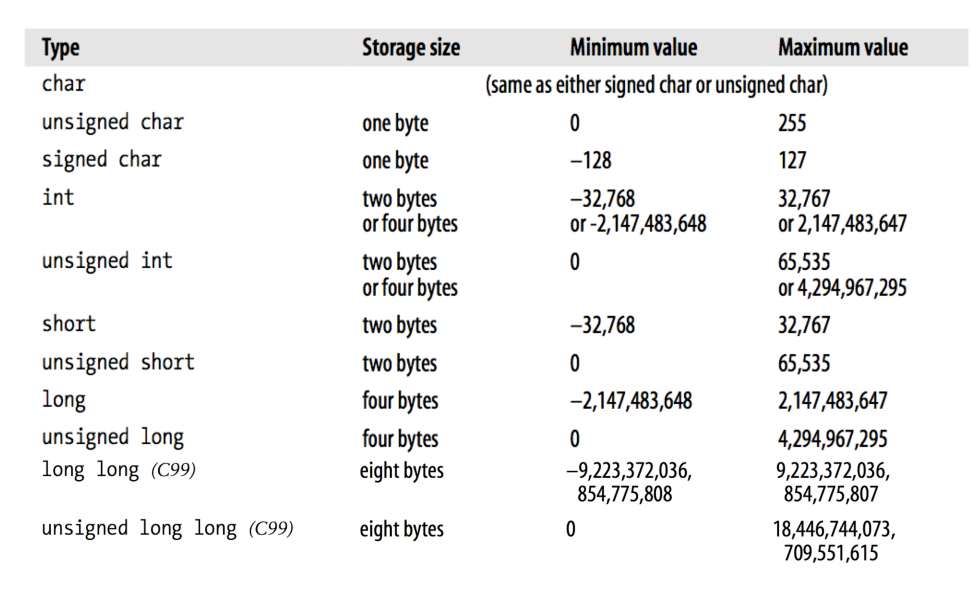
\includegraphics[width=13cm, keepaspectratio]{capitoli/secure_coding/img/cap_2/vari_tipi.png}
    \caption{Tabella raffigurante tutti i tipi in C con la loro dimensione.}\label{fig:vari_tipi}
\end{figure}

\subsection{Tipi unsigned}

Un calcolo che coinvolge operandi senza segno non può mai fare overflow.
Se un valore è fuori intervallo, viene eseguito il seguente calcolo:

\[
    toolargevalue \ mod \ MaxValue + 1
\]

Si ha un \textbf{wraparound} quando un valore sfora il massimo numero
rappresentabile. Di seguito vediamo gli operatori che possono o no avere
wraparound (a partire da operazioni con gli unsigned):

\begin{figure}[H]
    \centering
    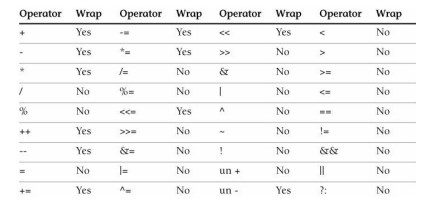
\includegraphics[width=10cm, keepaspectratio]{capitoli/secure_coding/img/cap_2/wraparound.png}
    \caption{Tabella raffigurante le operazioni che effettuano wraparound.}
\end{figure}

\subsection{Tipi signed}

In C, ogni tipo di numero intero unsigned, escluso \_Bool, ha un corrispondente
tipo di numero intero signed che occupa la stessa quantità di memoria.
Se non viene precisato, un valore viene automaticamente considerato signed
(non vale per il char).
I numeri interi con segno (\verb|signed int|) sono ottenuti utilizzando il \textbf{complemento a 2},
che permette di rappresentare sia numeri positivi
che negativi utilizzando 1 bit per il segno (il primo bit) e risolvendo il problema del doppio 0 aggiungendo
1 dopo aver fatto il complemento bit a bit.
Rappresentando 8 bit con il complemento a 2 avremmo un range che varia tra $-128$ a $127$.
In generale il range di rappresentazione sarà dato dalla seguente formula:
\[
    da \ -2^{N} - 1 \ \ a \ \ 2^{N - 1} - 1
\]

dove $N$ è il numero di bit.\\
Di seguito vediamo gli operatori che possono o no avere wraparound (a partire da
operazioni con i signed):

\begin{figure}[H]
    \centering
    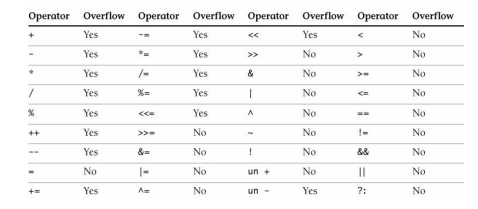
\includegraphics[width=12cm, keepaspectratio]{capitoli/secure_coding/img/cap_2/wraparound_signed.png}
    \caption{Tabella raffigurante le operazioni che effettuano wraparound su signed.}
\end{figure}

\subsection{Esempi}

\begin{figure}[H]
    \centering
    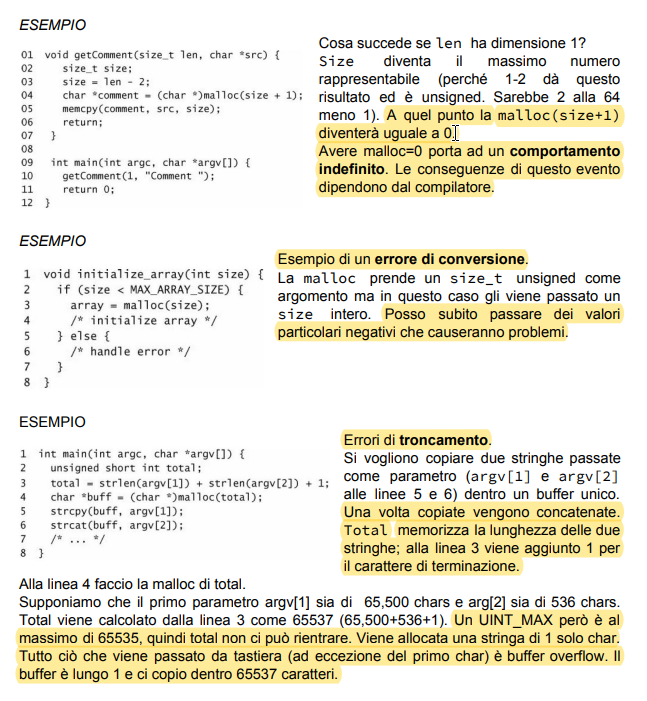
\includegraphics[width=12cm, keepaspectratio]{capitoli/secure_coding/img/cap_2/esempi.png}
\end{figure}

\section{Vulnerabilità degli Interi}

I potenziali problemi alla sicurezza causati dagli int provengono da errori di 3 tipi:

\begin{itemize}
    \item \textbf{Overflow/Wraparound}: occorre quando un'operazione genera valori
          che si trovano al di fuori del range di un particolare tipo di interi
    \item \textbf{Truncation}: occorre quando un valore viene salvato in un tipo
          troppo piccolo per rappresentarlo
    \item \textbf{Conversions}: sono errori generati da cast impliciti o espliciti
          in valori che si trovano al di fuori del range del tipo risultante.
\end{itemize}

Ci sono vari modi per prevenire tali errori:

\begin{itemize}
    \item \textbf{Integer Type Selection}:
          consiste nel selezionare il tipo più
          appropriato per il codice che si ha sotto mano.
          Un esempio è l'uso del tipo \verb|size_t| quando si vuole salvare la
          dimensione di un oggetto dato che ideato per questo scopo
          ("INT01-C. Use \verb|size_t| for all integer values representing the size of
          an object.").
          Si può anche utilizzare \verb|short|.\\
          Un esempio: \verb|size_t total = strlen(argv[1])+ 1;|\\
          Un altro esempio:
          \begin{figure}[H]
              \centering
              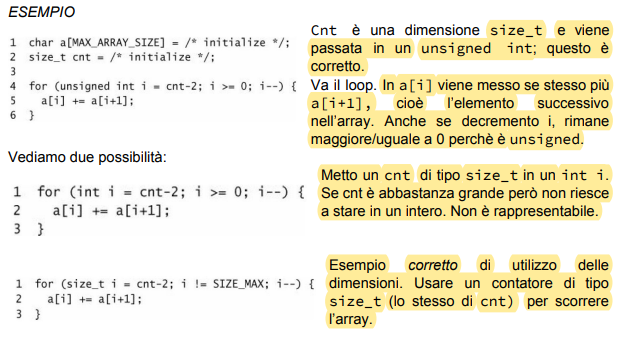
\includegraphics[width=12cm, keepaspectratio]{capitoli/secure_coding/img/cap_2/esempio_sizet.png}
          \end{figure}

    \item \textbf{Type Range Checking}:
          controlla se avvengono errori legati al superamento del range degli interi,
          alcuni modi per farlo solo: \begin{itemize}
              \item \textit{Pre-Conditions}:
                    questa tecnica si basa sul controllare la possibile presenza di
                    overflow o wrapping prima che un'operazione venga eseguita.
                    Di seguito un esempio:
                    \begin{lstlisting}
unsigned int ui1, ui2, usum;

// initialize ui1 and ui2

if (UINT_MAX - ui1 < ui2) {
    // handle error condition
}
else {
    usum = ui1 + ui2;
}
                    \end{lstlisting}
              \item \textit{Post-Conditions}:
                    è equivalente alla pre-condition ma viene eseguita dopo
                    l'esecuzione di un'operazione ed è in grado di controllare solo la
                    presenza di wrapping. Di seguito un esempio:
                    \begin{lstlisting}
    unsigned int ui1, ui2, usum;

    // initialize ui1 and ui2

    usum = ui1 + ui2;

    if (usum < ui1) {
        // handle error condition
    }
                    \end{lstlisting}
          \end{itemize}
    \item \textbf{Secure Integer Libraries}:
          sono presenti librerie sviluppate appositamente per gestire questi
          tipi di errori tramite meccanismi architecture-specific.
    \item \textbf{Compiler Checks}:
          GCC fornisce il flag \verb|-ftrapv| che crea delle trap per le
          operazioni di addizione, sottrazione e moltiplicazione con segno
          quando generano overflow a runtime.
    \item \textbf{Testing e Static Analysis}:
          effettuare procedure di Static Analysis,
          dal compilatore o un altro strumento apposito,
          per la detection di possibili errori nei range degli interi.
\end{itemize}

\section{Array e stringhe}

\paragraph{Problemi con gli array.}
Il  CERT C Secure Coding Standard include il fatto di non applicare
l'operatore \textit{sizeof} a un puntatore quando si vuole la grandezza dell'array.
Esempio:

\begin{figure}[H]
    \centering
    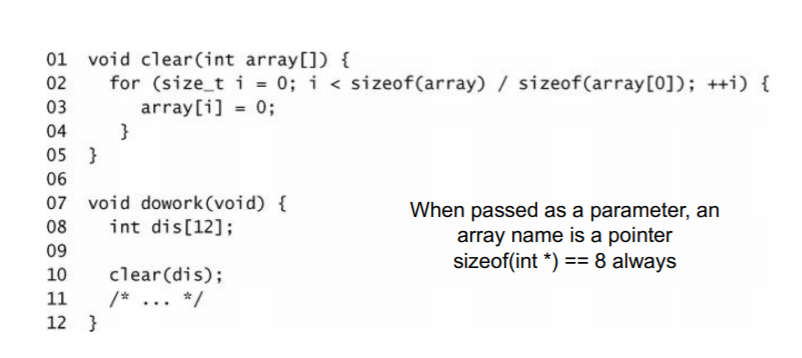
\includegraphics[width=10cm, keepaspectratio]{capitoli/secure_coding/img/cap_2/sizeof_array.png}
    \caption{Esempio \textit{sizeof(array)} .}\label{fig:sizeof_array}
\end{figure}

\paragraph{Stringhe.}
Le stringhe sono un concetto fondamentale nell'ingegneria del software,
ma essi non sono un tipo integrato in C o C++. Infatti la libreria standard di C
supporta le stringhe di tipo \verb|char| e le stringhe larghe di tipo \verb|wchar_t|.

\begin{figure}[H]
    \centering
    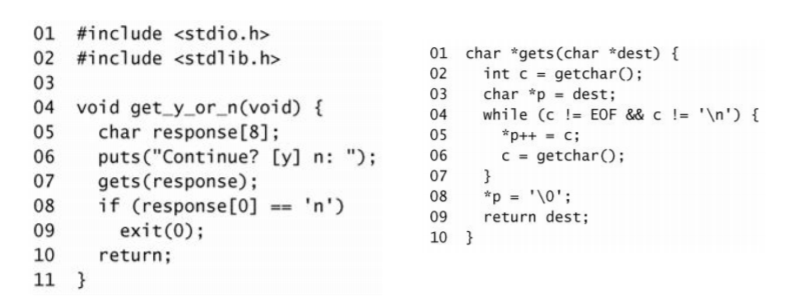
\includegraphics[width=10cm, keepaspectratio]{capitoli/secure_coding/img/cap_2/gets_1.png}
    \caption{Esempio \textit{gets} .}\label{fig:gets}
\end{figure}

Il problema principale con la funzione \verb|gets()| è che non fornisce alcun modo
di specificare un limite sul numero dei caratteri da leggere.
Quest'ultima risulta deprecata e eliminata, il CERT consiglia di non utilizzare
funzioni deprecate o obsolete.

\paragraph{Lettura da \textit{stdin()}.}
La lettura dei dati da una una fonte illimitata come \textbf{stdin()} crea dei
problemi per il programmatore poiché non è possibile conoscere in anticipo quanti
caratteri un utente utilizzerà, infatti è impossibile pre-allocare un array di
sufficiente lunghezza. Una soluzione comune è di allocare staticamente un array più
grande rispetto al necessario. Questo approccio funziona con gli utenti "amichevoli",
ma con gli attaccanti un array di caratteri di lunghezza fissa può essere facilmente
superato. Infatti questo metodo è proibito dal CERT il quale afferma che non si può
copiare dati da una fonte illimitata in un array con lunghezza fissata.\\
\textit{“STR35-C. Do not copy data from an unbounded
    source to a fixed-length array.”}

\paragraph{Parametri dei programmi.}
Le vulnerabilità possono occorrere quando uno spazio inadeguato è allocato per
copiare un input di un programma come un argomento della riga di comando.

\begin{figure}[H]
    \centering
    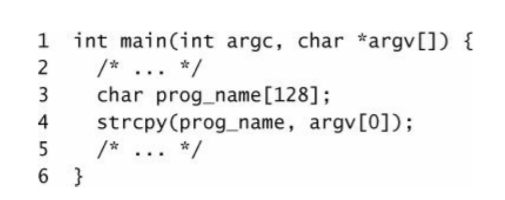
\includegraphics[width=10cm, keepaspectratio]{capitoli/secure_coding/img/cap_2/parametri_funzioni.png}
    \caption{Esempio vulnerabilità con parametri dei programmi .}\label{fig:parametri_programmi}
\end{figure}

Nonostante \verb|argv[0]| contiene il nome del programma, un attaccante può
controllare il contenuto di \verb|argv[0]| per causare una vulnerabilità fornendo
una stringa con più di 128 bytes.

\paragraph{Null terminating string.}
In Figura \ref{fig:null_string} possiamo vedere che il risultato di \verb|strcpy()|
su c porta l'utente a poter scrivere oltre i limiti dell'array poiché la stringa
salvata in \verb|a[]| non terminata correttamente (null-terminating).


\begin{figure}[H]
    \centering
    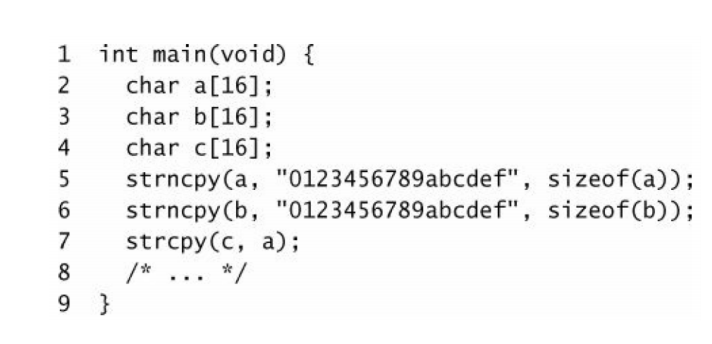
\includegraphics[width=10cm, keepaspectratio]{capitoli/secure_coding/img/cap_2/null_string.png}
    \caption{Esempio null terminating string .}\label{fig:null_string}
\end{figure}

\textit{“STR32-C. Null-terminate byte strings as
    required.”}

\paragraph{Funzionamento esempio \ref{fig:null_string}}
Abbiamo 3 array lunghi 16 caratteri, copiamo la stringa "0123456789abcdef"
in \textbf{a} e in \textbf{b}, come si può notare questa stringa ha una lunghezza di
16 caratteri. Successivamente si copia la stringa contenuta in \textbf{a}
nell'array \textbf{c} e questo porta ad avere dei problemi ovvero:

\begin{itemize}
    \item non viene salvato sia in \textbf{a} che in \textbf{b} il carattere di fine
          stringa "\textbackslash0" allora essendo che la stringa non termina
          e che 'array \textbf{b} è memorizzato subito dopo \textbf{a} si ha di conseguenza che
          \[a = [0123456789abcde0123456789abcde\backslash 0]\]
    \item quindi quando si va a copiare \textbf{a} dentro \textbf{c} si copiano 32
          caratteri più "\textbackslash0" e non 16 sforando così la memoria allocata inizialmente.
\end{itemize}

\section{Vulnerabilità delle stringhe ed exploit}

\subsection{Valori corrotti}

Precedentemente abbiamo visto alcuni degli errori più comuni nel manipolare il
linguaggio C o C++. Questi errori sono pericolosi nel momento in cui il codice opera
con dati esterni non fidati come gli argomenti delle linee di comando, variabili
d'ambiente, input della console, file di testo e connessione a internet.
\textbf{Infatti è meglio considerare tutti i dati esterni al codice come non fidati. }
Nell'analisi della sicurezza dei software, un valore è
chiamato \textbf{corrotto (tainted)} quando viene da una risorsa non fidata, al di
fuori del controllo del programma, e non \textbf{è stato sanificato} per assicurarsi
che sia conferme a qualsiasi vincolo posto su di esso.

\begin{figure}[H]
    \centering
    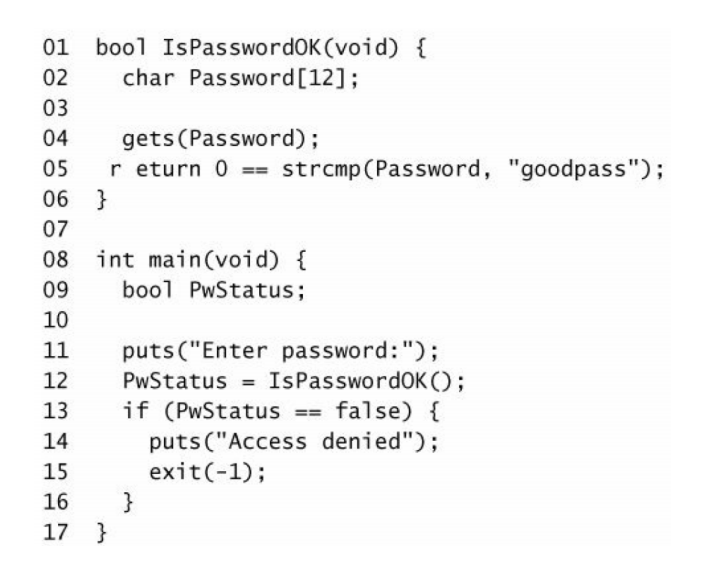
\includegraphics[width=10cm, keepaspectratio]{capitoli/secure_coding/img/cap_2/password_example.png}
    \caption{Esempio password.}\label{fig:password}
\end{figure}

\subsection{Buffer overflow.}

In questo caso la falla sta nella funzione \verb|IsPasswordOk()| poiché permette ad
un attaccante di guadagnare l'accesso non autorizzato causato dalla
funzione \verb|gets()|. Questa tipologia di attacco che permette una scrittura oltre
i limiti viene definita \textbf{buffer overflow}.

\begin{figure}[H]
    \centering
    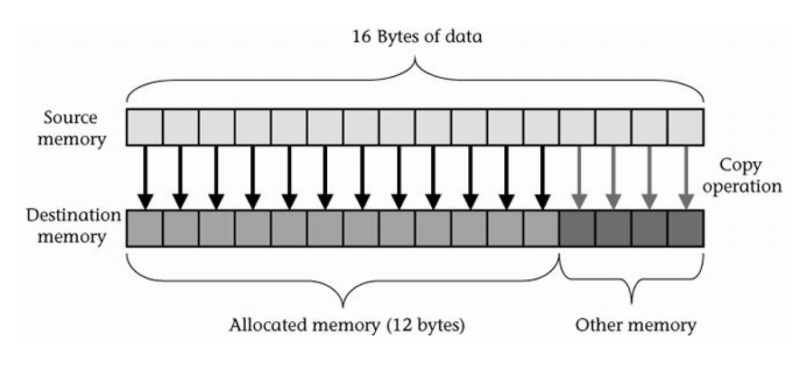
\includegraphics[width=10cm, keepaspectratio]{capitoli/secure_coding/img/cap_2/memory.png}
    \caption{Allocazione della memoria.}\label{fig:memoria}
\end{figure}

Oltre questo è presente anche un altro problema ovvero che il
programma \verb|IsPasswordOk| non controlla lo stato di ritorno di \verb|gets|. \\
\textit{“FIO04- C. Detect and handle input and output errors.”}\\
Quando si fallisce l'inserimento della password non viene controllato da nessuno
perciò il contenuto del buffer \verb|Password| è indeterminato, nei programmi reali
esso potrebbe contenere la password del precedente utente.
Il buffer overflow occorre quando un dato è scritto oltre i limiti della memoria
allocata in una particolare struttura. Il linguaggio C e C++ sono
suscettibili a questi attacchi poiché:

\begin{itemize}
    \item Definisce le stringhe come array di caratteri con terminazione null;
    \item Non usano dei metodi per il controllo implicito dei limiti;
    \item Fornisce funzioni per le stringhe che non applicano dei controlli.
\end{itemize}

Non tutti i buffer overflow portano a delle vulnerabilità, solo nel caso in cui un
attaccante può manipolare gli input controllati dall'utente per sfruttare una
falla di sicurezza.\\
Il buffer overflow può essere sfruttato sia nella memoria \textbf{heap} che in
quella \textbf{statica} sovrascrivendo strutture di memoria adiacenti.
Per aiutare nel verificare la presenza di un buffer overflow esistono dei programmi
che a tempo di compilazione (\textbf{staticamente}) o in modo \textbf{dinamico}
(eseguono il programma passando delle stringhe dove viene richiesto) controllano la
presenza o meno di quest'ultimi.

\section{Memoria}

\subsection{Organizzazione di un processo in memoria}

Nell'immagine sottostante possiamo vedere come è organizzata la memoria in 3
differenti casi, il primo è il caso generale che andremo a prendere in considerazione,
il secondo riguarda la memoria in Linux e l'ultimo in Windows.

\begin{figure}[H]
    \centering
    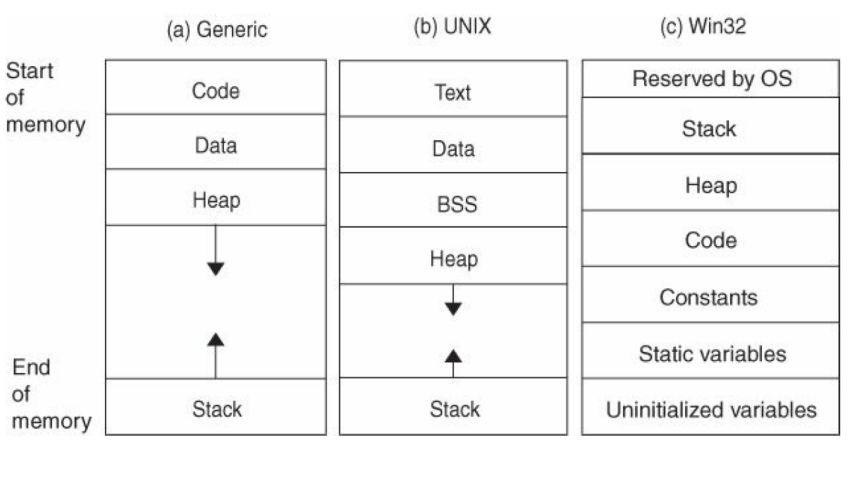
\includegraphics[width=10cm, keepaspectratio]{capitoli/secure_coding/img/cap_2/memoria.png}
    \caption{Organizzazione della memoria.}\label{fig:org_memoria}
\end{figure}

Studiamo le varie parti della memoria nel caso generale:

\begin{itemize}
    \item \textbf{Code}: zona in cui viene salvato il codice del programma;
    \item \textbf{Data}: memoria  in cui sono salvate le variabili globali e le
          variabili locali statiche, inizializzate e non;
    \item \textbf{Heap:} memoria per allocazione dinamica dei processi, gli indirizzi
          di memoria aumentano in modo crescente;
    \item \textbf{Stack:} zona LIFO (pila) in cui vengono salvate le variabili locali
          alle funzioni (supporto per l'esecuzione dei processi), gli indirizzi di memoria
          aumentano in modo decrescente .
\end{itemize}

Noi vedremo degli esempi di buffer overflow nello stack, è molto importante ricordarsi
come funziona e come vengono salvate le variabili, se si alloca dello spazio si va da
un numero più alto a uno più basso e viceversa (come una fisarmonica). La memoria è
struttura in questo modo così la parte dinamica (heap) non si incontra con la parte
statica (stack) a meno che non viene riempita completamente.\\
La memoria UNIX è molto simili alla memoria generale, l'unica differenza sta nel
fatto che la parte \textbf{Data} nella memoria generale viene suddivisa in due in
quella UNIX:

\begin{itemize}
    \item \textbf{Data:} vengono salvate delle variabili globali/statiche
          inizializzate;
    \item \textbf{BSS(Block Started by Symbol):} vengono salvate le variabili globali
          che non sono state inizializzate e vengono di default inizializzate a 0.
\end{itemize}

Il segmento \textbf{Text} è l'equivalente del segmento \textbf{Code}, entrambi
includono le istruzioni e i dati read-only.

\paragraph{Esecuzione di un programma.}
Vediamo un primo esempio di esecuzione di un programma.
In questo caso possiamo vedere due funzioni \verb|main()| e \verb|fun(...)|, si parte
salvando in memoria le variabili locali presenti nella funzione \verb|main()| la
quale richiama l'altra. In Figura \ref{fig:es_esec_processo} possiamo vedere che le
variabili vengono salvate in sequenza dal basso verso l'alto in base a come sono state
inizializzate, successivamente con la chiamata di \verb|fun()| si salvano i parametri
che essa prende in input, l'indirizzo di
ritorno (\textbf{return address}\footnote{indica l'indirizzo di ritorno dopo che è
    stata eseguita la funzione in questione, in questo caso indica l'indirizzo del main.})
e la variabile res. Il segmento che contiene la variabile del main si
chiama \textbf{stack/frame main}, stessa definizione per il segmento di fun.
Al termine dell'esecuzione di fun si cancella dalla memoria tutto quello riguardante
quest'ultima e si ritorna all'istruzione successiva alla chiamata di funzione in main.
Per riportare il controllo nella posizione corretta, deve essere salvato l'indirizzo
di ritorno. Lo stack è adatto a mantenere queste informazioni perché è una struttura
dati dinamica in grado di supportare qualsiasi livello di annidamento all'interno
vincoli di memoria.

\begin{figure}[H]
    \centering
    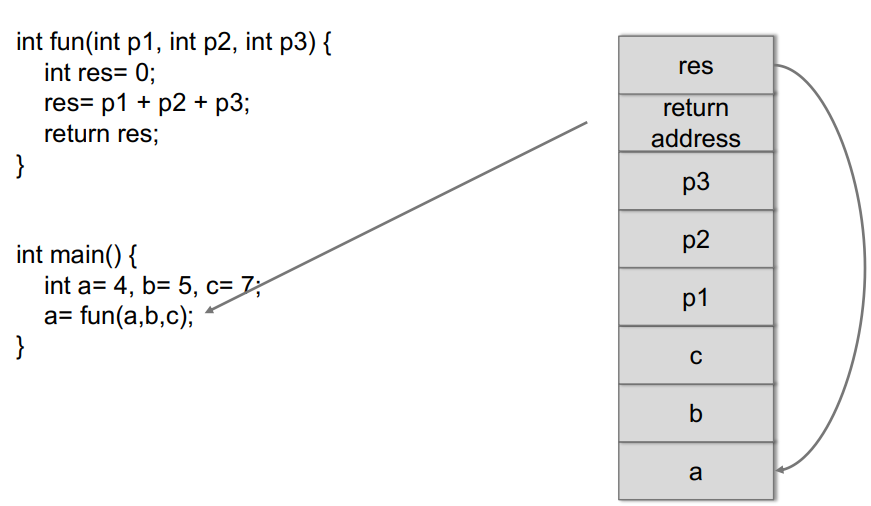
\includegraphics[width=13cm, keepaspectratio]{capitoli/secure_coding/img/cap_2/es_esecuzione_processo.png}
    \caption{Esempio esecuzione processo.}\label{fig:es_esec_processo}
\end{figure}

\subsection{Puntatori}

\subsubsection{Extended base pointer (EBP)}

L'indirizzo del frame corrente è salvato all'interno del frame o
nel \textbf{base pointer register}.
Il registro \textbf{extended base pointer (ebp) } è usato per questo scopo, esso è
usato anche come punto fissato di riferimento all'interno dello stack. Quando una
subroutine è chiamata, il puntatore del frame per la routine di chiamata viene anch'esso
inserito nello stack in modo che può essere ripristinato quando la subroutine termina.

\subsubsection{Instruction pointer}

Il \textbf{puntatore di istruzione (eip)} punta all'istruzione successiva da eseguire,
quando si esegue una sequenza di istruzioni esso è aumentato automaticamente dalla
grandezza di ogni istruzioni. Eip non può essere modificato direttamente ma deve
essere modificato indirettamente con delle istruzioni come:

\begin{itemize}
    \item jump;
    \item call;
    \item return.
\end{itemize}

\subsubsection{Extended stack pointer (ESP)}

L'\textbf{extended stack pointer (esp)} è il puntatore corrente allo stack, esso
punta alla parte superiore della pila.

\section{Stack overflow}

\paragraph{Secondo esempio}
In questo secondo esempio possiamo vedere che ci sono 3 funzioni
(\verb|main|, \verb|f1| e \verb|f2|) che si chiamano a vicenda.
Quando viene eseguito il programma viene inserito nello stack il frame del \verb|main|,
supponiamo che esso inizi dall'indirizzo 1000, il quale viene salvato all'interno
del ebp e del registro della CPU. Successivamente quando viene chiamata la
funzione \verb|f1| l'ebp all'interno del registro della CPU cambia con quello
dell'inizio del frame di \verb|f1|, ovvero 1008.
All'interno del frame di \verb|f1| vengono salvati oltre alle variabili locali
anche il valore del ebp corrente(1008) e il valore di ritorno, il quale è uguale
all'epb del \verb|main| poiché appena terminata \verb|f1| la CPU deve tornare a
eseguire le istruzioni successive alla chiamata di funzione nel frame \verb|main|.

\begin{figure}[H]
    \centering
    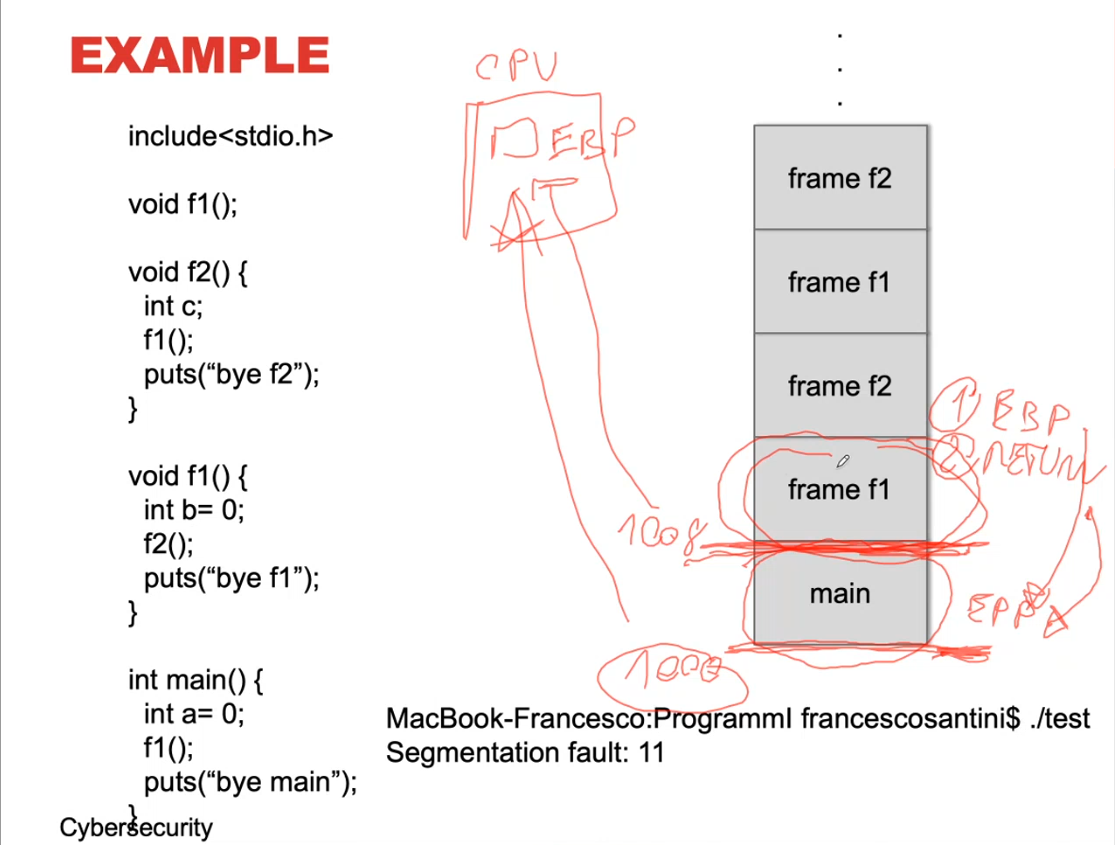
\includegraphics[width=13cm, keepaspectratio]{capitoli/secure_coding/img/cap_2/es_process_spiegato.png}
    \caption{Esempio esecuzione processo con spiegazione.}\label{fig:es_esec_processo2}
\end{figure}

\paragraph{Esempio disassembly in intel.} Adesso vediamo cosa succede a livello assembly
\footnote{Il linguaggio assembly (detto anche linguaggio assemblativo o linguaggio
    assemblatore o semplicemente assembly) è un linguaggio di programmazione molto simile al
    linguaggio macchina, pur essendo differente rispetto a quest'ultimo.} quando si
chiama una funzione. La funzione \verb|main| alloca due variabili \verb|MyInt|
(intero, 4 byte) e \verb|*MyStrPtr| (puntatore a carattere, 4 byte), poi chiama la
funzione \verb|foo| a cui vengono passati come parametri le variabili definite prima.
Ci sono degli errori fra la spiegazione del professore e i commenti nell'esempio,
ovvero MyInt come parametro viene allocato per primo nello stack secondo il professore
mentre nel commento a riga 4 viene allocato come secondo rispetto a MyStrPtr poiché gli
argomenti delle funzioni vengono allocati da destra verso sinistra, per comodità seguiamo
la spiegazione delle slides.
A livello assembly quando viene chiamata la funzione vengono effettuate le seguente operazioni,:

\begin{enumerate}
    \item  \verb|mov eax, [ebp- 4]|: si sposta quello che si trova in ebp-4 (MyStrPtr)
          in eax, dove ebp = 1000 e ebp-4 = 996;
    \item \verb|push eax|: si inserisce eax (MyStrPtr) nello stack;
    \item  \verb|mov ecx, [ebp- 8]|: si sposta quello che si trova in
          ebp-8 (MyInt) in ecx,  dove ebp = 1000 e ebp-8= 992;
    \item \verb|push ecx|: si inserisce ecx (MyStrPtr) nello stack;
    \item \verb|call foo|: chiamiamo la funzione \verb|foo| e inseriamo nello stack
          il return address in cima al frame di foo;
    \item \verb|add esp, 8|: aggiunge 8 byte al puntatore esp dopo il return di foo.
\end{enumerate}

\begin{figure}[H]
    \centering
    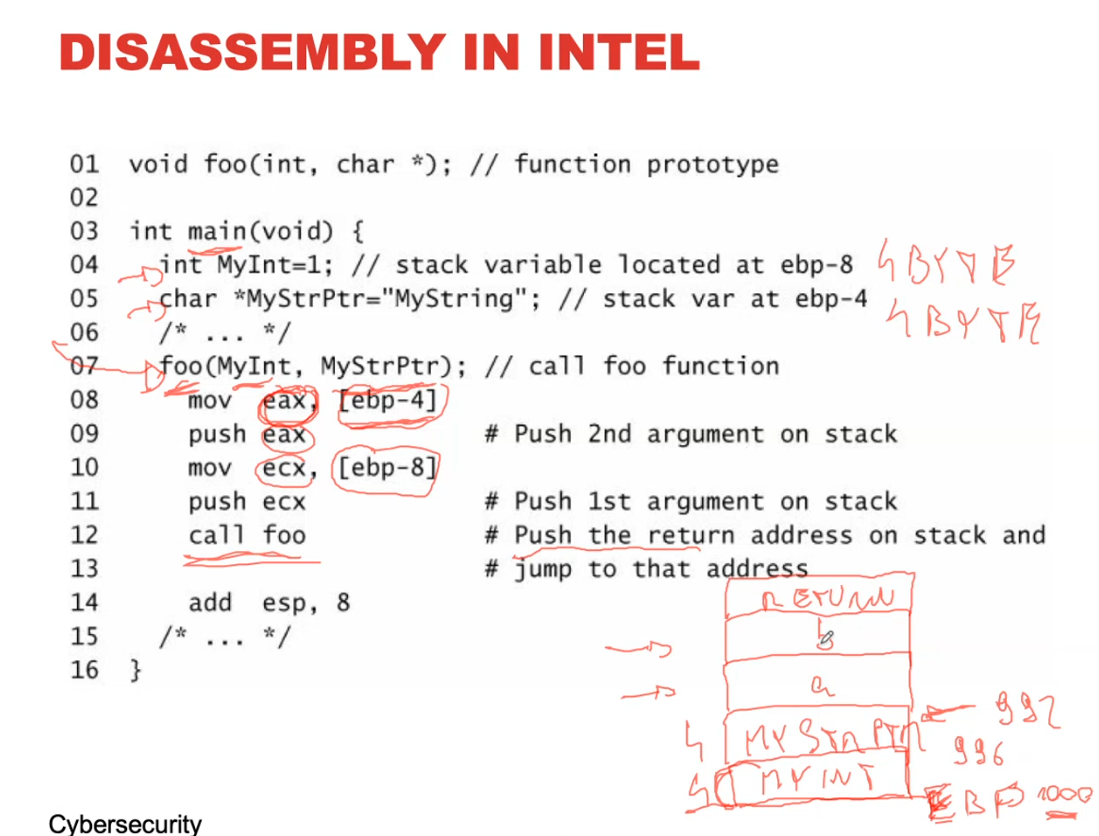
\includegraphics[width=13cm, keepaspectratio]{capitoli/secure_coding/img/cap_2/disass_intel_1.png}
    \caption{Esempio disassembly main in intel.}\label{fig:disass_intel_1}
\end{figure}

Vediamo ora come si comporta la funzione \verb|foo| quando viene chiamata,
Figura \ref{fig:disass_intel_2}. Dopo aver salvato il return address salviamo anche
l'ebp della funzione \verb|main| in modo da ricordarsi dove inizia il suo frame
quando la chiamata di funzione \verb|foo| termina. Dopo ebp di main inizia il
frame di \verb|foo| dove verranno salvate tutte le sue variabili locali,
esso è grande 28 byte.

\begin{enumerate}
    \item \verb|push ebp|: salva il puntatore al frame corrente ovvero ebp di main;
    \item \verb|mov ebp, esp|: salviamo il puntatore alla fine del frame di main
          esp nel ebp, in modo da iniziare il frame di foo alla fine di quello del main;
    \item \verb|sub esp, 28|: allochiamo 28 byte di spazio per foo con esp - 28.
\end{enumerate}

\begin{figure}[H]
    \centering
    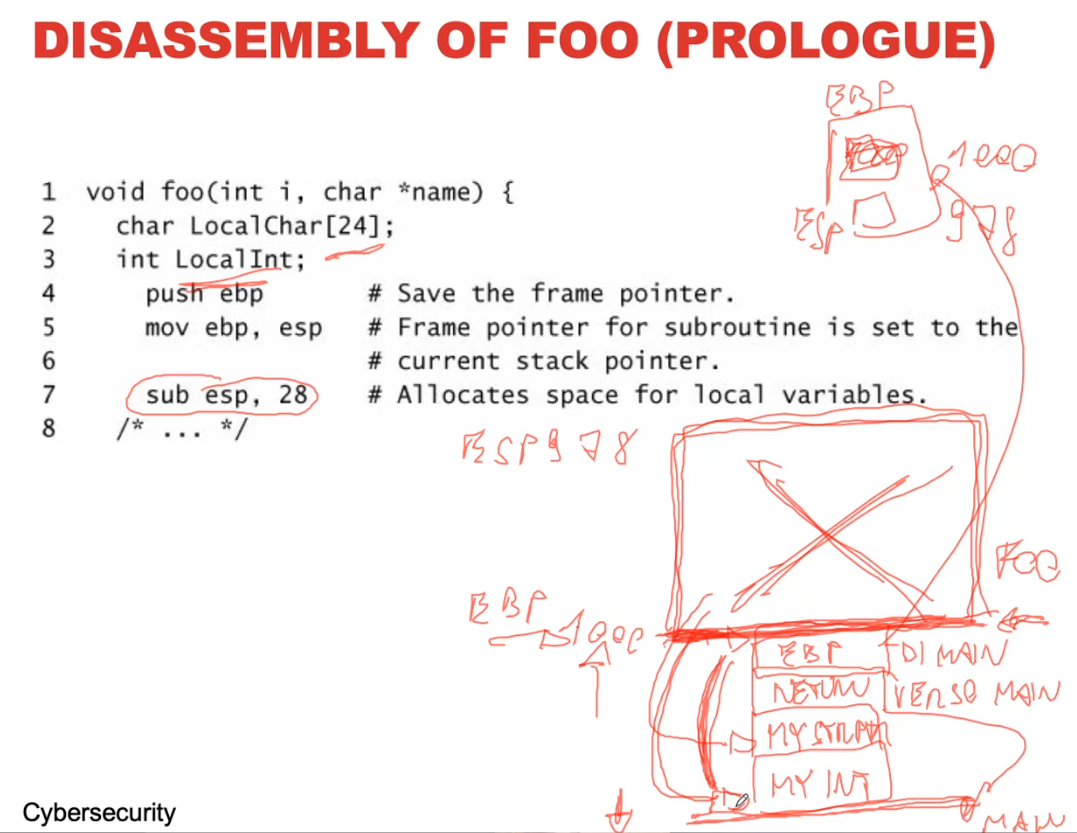
\includegraphics[width=13cm, keepaspectratio]{capitoli/secure_coding/img/cap_2/disass_intel_2.png}
    \caption{Esempio disassembly foo in intel.}\label{fig:disass_intel_2}
\end{figure}

Come si può vedere anche nell'immagine sottostante, il frame di foo è costituito dai
seguenti elementi in questo ordine:

\begin{enumerate}
    \item Primo parametro della funzione foo: \verb|toMyString| (4 byte);
    \item Secondo argomento: \verb|MyInt| (4 byte);
    \item Return address del main (4 byte);
    \item Ebp del main (4 byte);
    \item Prima variabile locale \verb|LocalChar| (24 byte);
    \item Seconda variabile locale \verb|LocalInt|  (4 byte).
\end{enumerate}

\begin{figure}[H]
    \centering
    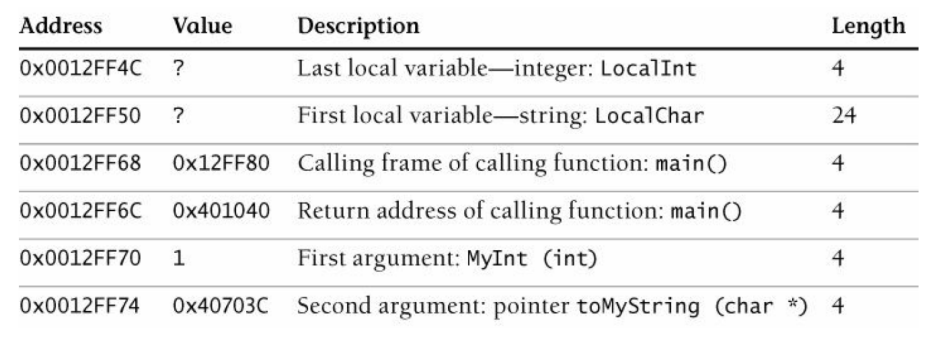
\includegraphics[width=13cm, keepaspectratio]{capitoli/secure_coding/img/cap_2/diss_stack.png}
    \caption{Frame di foo.}\label{fig:frame_foo}
\end{figure}

Infine vediamo cosa succede quando facciamo il return di foo, in generale lo scopo
è di disallocare tutto lo spazio di memoria della funzione foo e di tornare
all'istruzione successiva del main. Esso è composto da più comandi in assembly che sono:

\begin{enumerate}
    \item \verb|mov esp,ebp|: allo stack pointer esp inserisco il valore del ebp del
          frame corrente, ovvero si passa ad esempio da esp = 900 $\rightarrow$1000.
    \item \verb|pop ebp|: ristabilisce il frame pointer ebp con quello della funzione
          chiamante (main), ovvero disallocando i 28 byte del frame di foo il primo
          elemento che troviamo in memoria è proprio il valore del ebp del main che ci
          eravamo salvati in precedenza, facendo il pop lo eliminiamo dalla pila e lo
          reinseriamo nel registro della CPU;
    \item \verb|ret|: fa il pop del return address dallo stack, lo mette nel
          eip (prossima istruzione da fare ovvero tornare al punto di chiamata) e
          trasferisce il controllo a quel frame.
\end{enumerate}

Dopo aver fatto il return si esegue il prossimo comando che è appunto \verb|add esp, 8|
in Figura \ref{fig:disass_intel_1}, il quale aggiunge all'esp 8 byte perché dalla
memoria devono essere eliminati ancora i parametri passati alla funzione chiamata
che sono MyStrPtr e MyInt. In questo modo si torna l'esp combacia con la parte alta
del frame del main e l'ebp con l'inizio di quest'ultimo.

\begin{figure}[H]
    \centering
    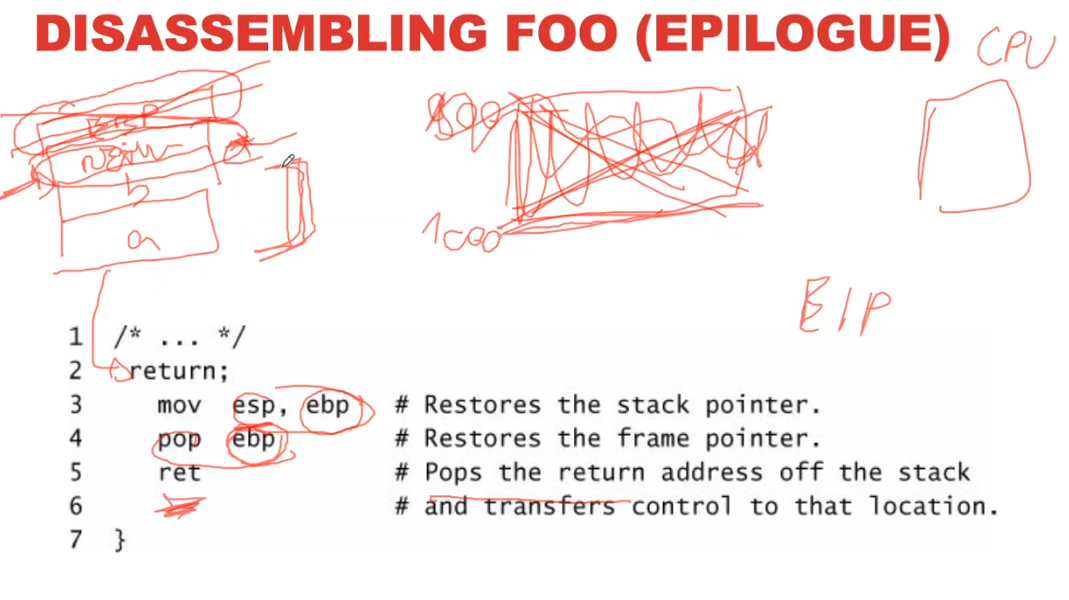
\includegraphics[width=13cm, keepaspectratio]{capitoli/secure_coding/img/cap_2/disass_intel_3.png}
    \caption{Return di foo.}\label{fig:disass_intel_3}
\end{figure}

\paragraph{Valori di ritorno.} Se ci sono dei valori di ritorno questi sono salvati
in eax dalla funzione chiamata prima che ritorni al main. In questo modo la
funzione chiamante sa dove si trovano i valori di ritorno e li può usare.

\begin{figure}[H]
    \centering
    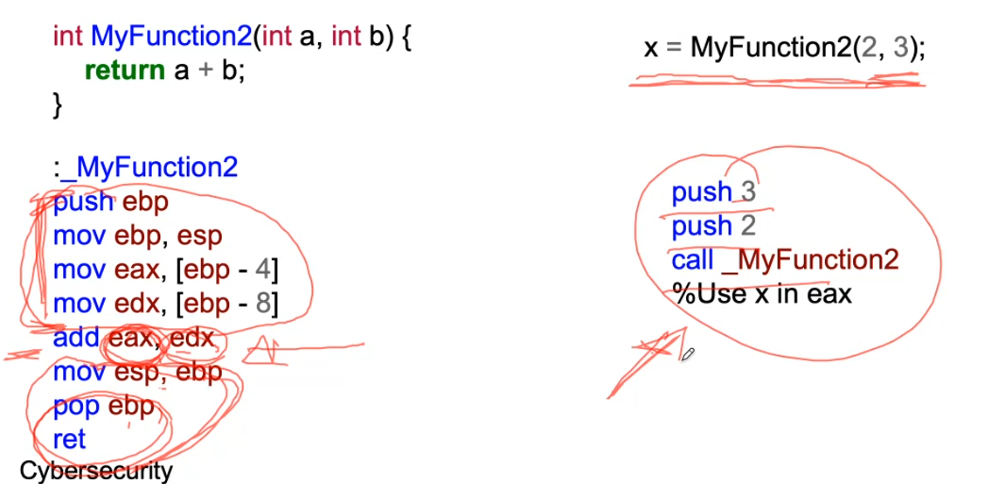
\includegraphics[width=13cm, keepaspectratio]{capitoli/secure_coding/img/cap_2/return_values.png}
    \caption{Valori di ritorno.}\label{fig:ret_values}
\end{figure}

\section{Stack smashing}

Stack smashing è quando un attaccante intenzionalmente fa overflow di un buffer nello
stack per ottenere l'accesso a vietato regioni della memoria del computer.
Questo avviene quando si riscrivono dei dati all'interno della memoria allocata
all'esecuzione dello stack. Si possono avere delle serie conseguenze come ad esempio
la modifica di valori delle \textbf{variabili automatiche} o l'esecuzione di codice
arbitrario. Un esempio comune è sovrascrivere il return address che si trova nello
stack.

\subsection{Arc Injection}

\subsubsection{Esempio \textit{IsPasswordOk}: Arc Injection}

Nell'esempio in Figura \ref{fig:password} il programma è vulnerabile a stack smashing.
Questo difetto può essere facilmente dimostrato inserendo una password di 20 caratteri
“1234567890123456 W$\triangleright$*!” che porta a far saltare il programma in modo
imprevisto.

\begin{figure}[H]
    \centering
    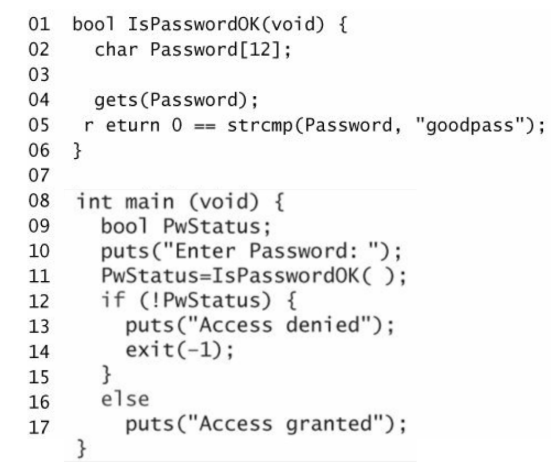
\includegraphics[width=8cm, keepaspectratio]{capitoli/secure_coding/img/cap_2/pass_ok_new.png}
    \caption{IsPasswordOk nuova.}\label{fig:pass_ok_new}
\end{figure}

\begin{figure}[H]
    \centering
    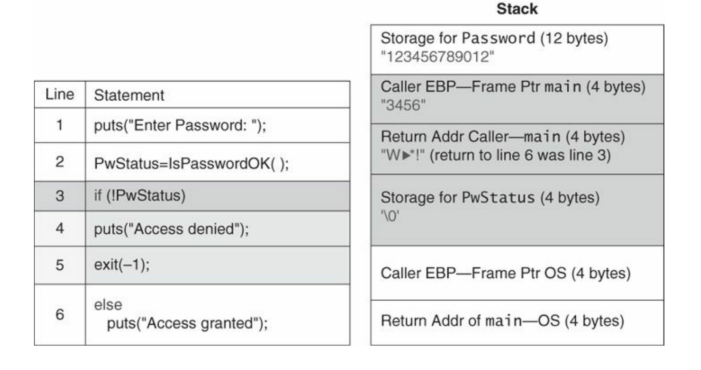
\includegraphics[width=13cm, keepaspectratio]{capitoli/secure_coding/img/cap_2/es_pass_ok_new.png}
    \caption{Funzionamento stack smashing.}\label{fig:es_pass_ok_new}
\end{figure}

In memoria l'ultima sequenza di quattro caratteri W$\triangleright$*! corrisponde a
un indirizzo di 4 byte che sovrascrive l'indirizzo di ritorno nello stack, quindi
invece di tornare all'istruzione subito dopo la chiamata in main() ritorna al ramo
“Access granted” bypassando così il controllo della password e autorizzando ad avere
accesso al sistema.
Un metodo per capire dove è salvato il return address di una funzione nello stack è
l'utilizzo del comando
\verb|void * __builtin_return_address (unsigned int level)| il quale permette di con
un valore di 0 di avere il return address della funzione corrente e con un valore di
1 ritorna il valore della funzione chiamante. Questa tecnica di buffer overflow si
chiama \textbf{Arc Injection}.


La tecnica di \textbf{Arc Injection} (a volte chiamata \textbf{return into-libc}) prevede
il trasferimento del controllo al codice esiste già nella memoria di processo.
Questi exploit sono chiamati così perché inseriscono un nuovo arco
(trasferimento del flusso di controllo) nel flusso di controllo del programma invece
di iniettare nuovo codice. Questa tecnica è preferita rispetto al code injection
per vari motivi:

\begin{itemize}
    \item Si utilizza del codice che si trova già in memoria nel sistema preso di mira,
          in questo modo le \textbf{impronte lasciate dall'attaccante sono significativamente minori};
    \item Essendo che questo metodo si basa su codice
          esistente, n\textbf{on può essere bloccato da schemi di protezione basati sulla memoria}
          come la creazione di segmenti di memoria non eseguibile.
\end{itemize}

\subsection{Code Injection (Shell Code)}

Quando l'indirizzo di ritorno viene sovrascritto a causa di un software difetto,
raramente indica istruzioni valide. Per un attaccante è possibile creare delle
stringhe speciali che contengono \textbf{un puntatore a qualche codice malevolo},
sempre creato dall'attaccante. Questo implica che quando il return address sovrascritto
viene invocato il controllo è trasferito al codice iniettato, il quale viene
eseguito con i permessi del programma. Per questo i programmi che vengono eseguiti
con permessi di \textbf{root} o dei \textbf{privilegi elevati} sono il target di
certi attacchi, infatti frequentemente il codice malevolo apre una shell remota
\textbf{(shellcode)} nella macchina compromessa permettendo all'attaccante di inserire
dei comandi.

\subsubsection{Esempio \textit{IsPasswordOk}: Code Injection.}

Prendendo sempre come esempio il programma "IsPasswordOk" \ref{fig:pass_ok_new}.

\begin{figure}[H]
    \centering
    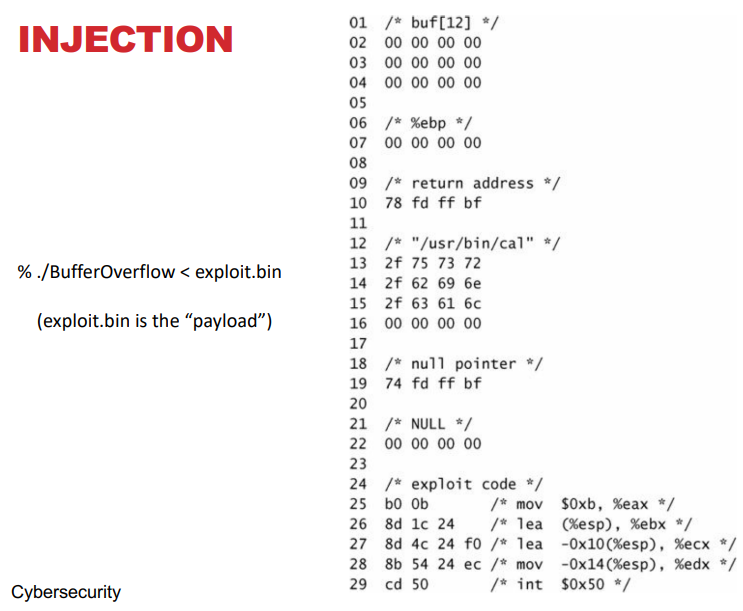
\includegraphics[width=12cm, keepaspectratio]{capitoli/secure_coding/img/cap_2/es_pass_ok_code_inj.png}
    \caption{Esempio con Code Injection}\label{fig:es_pass_ok_code_inj}
\end{figure}

Anche in questo caso cerchiamo di sovrascrivere il segmento del return address in modo
da farlo puntare al nostro codice malevolo che possiamo vedere al commento "exploit code".
Il nostro payload, ovvero il nostro codice, è tutto scritto in esadecimale per comodità
invece che in binario. Partiamo inserendo 12 caratteri nella variabile "Password"
successivamente sovrascriviamo il puntatore ebp con 4 interi casuali, non ci interessa
questa zona. Arriviamo infine al punto che ci interessa ovvero il segmento del return
address nel quale inseriremo come valore l'esadecimale del segmento dove salviamo
il codice di exploit in modo da eseguirlo. Prima di eseguire quest'ultimo salviamo 3
parametri che passeremo successivamente alle funzioni del exploit:

\begin{itemize}
    \item \textbf{"/usr/bin/cal"}: il primo esadecimale si traduce con il
          comando \verb|/usr/bin/cal|.
    \item \textbf{"null pointer"}: il secondo è un puntatore a null.
    \item \textbf{"NULL"}: caratteri nulli.
\end{itemize}

\textbf{Spiegazione exploit code.} Vediamo nel dettaglio cosa fanno i comandi scritti
in esadecimale del nostro exploit code.

\begin{itemize}
    \item \verb|mov $0xb, %eax|: assegna 0xB, il quale identifica il numero della chiamata
          di sistema \verb|execve()|, al registro \%eax; \\
          \begin{lstlisting}[language=C]
    int execve(
        const char *filename, 
        char *const argv[], 
        char *const envp[]
    );\end{lstlisting}
    \item \verb|lea (%esp), %ebx|: "load effective address", calcola l'indirizzo
          effettivo del secondo operando (operando sorgente) e lo salva nel primo (operando destinatario).
          L'operando sorgente è un indirizzo di memoria (parte offset) specificato con una delle
          modalità di indirizzamento del processore mentre l'operando di destinazione è un
          registro di uso generale. In questo caso vengono inseriti i tre parametri,
          salvati in precedenza agli
          indirizzi (\%esp), -0x10(\%esp) (esp-16) e -0x14(\%esp)(esp-20), nei registri
          ebx, ecx ed edx.
          \item\verb|int 0x50|: chiamata vera e propria  per invocare execve(), che
          comporta l'esecuzione del programma di calendario Linux.
\end{itemize}

\begin{figure}[H]
    \centering
    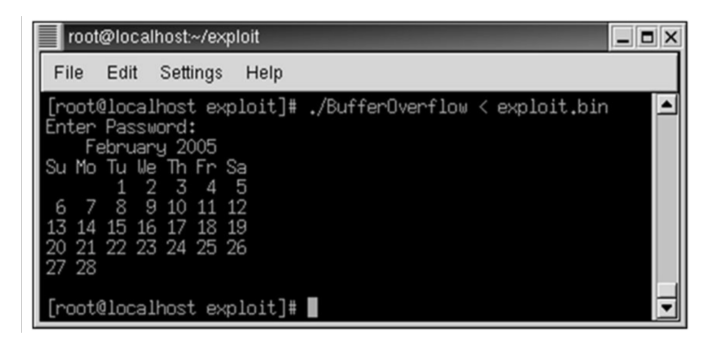
\includegraphics[width=12cm, keepaspectratio]{capitoli/secure_coding/img/cap_2/risultato_ex_pass_code_inj.png}
    \caption{Risultato esempio Code Injection.}\label{fig:ris_es_pass_ok_code_inj}
\end{figure}




